\subsubsection{Descrizione generale}
Questo servizio implementa le funzionalità di scraping ed in generale ottenimento dati da Instagram
e altre piattaforme ad esso correlate. Data la natura fondamentale ai fini del progetto, del compito
svolto da questo servizio, la complessità dell'implementazione è più alta rispetto agli altri servizi.

\subsubsection{Diagramma delle classi}
\begin{figure}[H]
    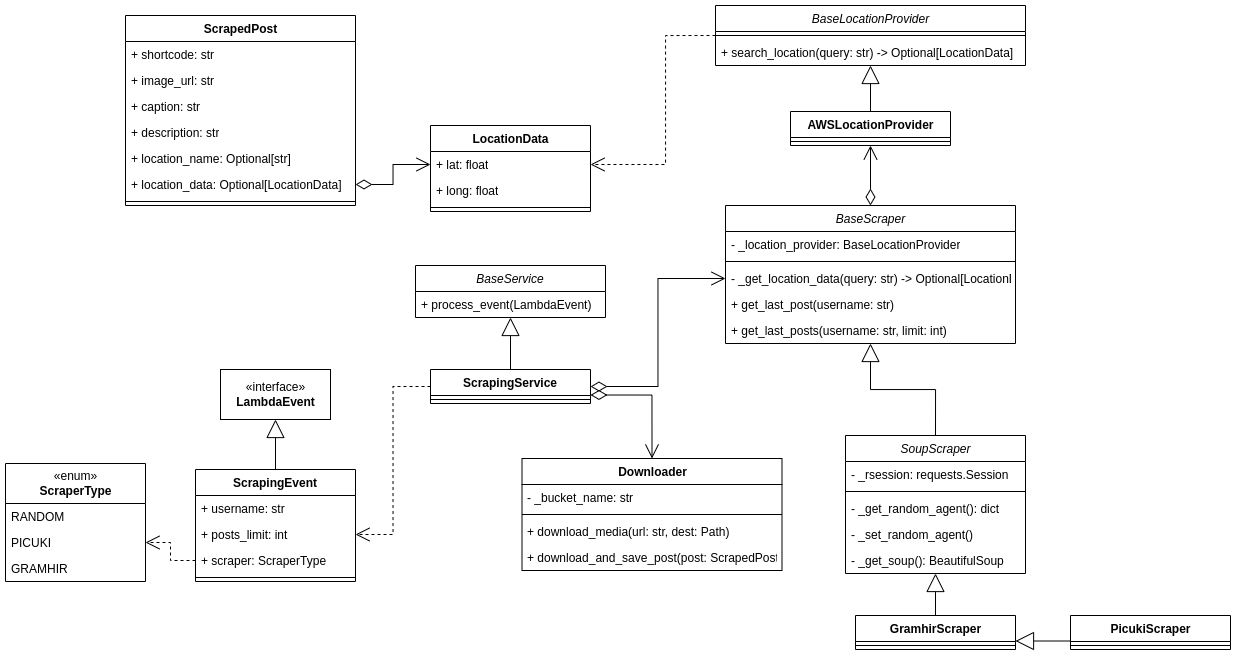
\includegraphics[width=14cm]{sezioni/images/cd_scraping.png}
    \centering
    \caption{Scraping Service - Diagramma delle classi}
\end{figure}

\subsubsection{Schemi I/O}
\paragraph*{Input} esempio di evento in input, in formato JSON\G{}.
\begin{lstlisting}[language=JSON]
{
    "username": "antoniorazzi",
    "posts_limit": 10
}
\end{lstlisting}
Descrizione:
\begin{itemize}
    \item \verb|username|: username del profilo social da cui effettuare lo scraping;
    \item \verb|posts_limit|: numero massimo di post di cui effettuare lo scraping. 
\end{itemize}

\paragraph*{Output} esempio di risposta in output, in formato JSON\G{}.
\begin{lstlisting}[language=JSON]
{
    "posts_count": 2,
    "posts": [
        {"id": 4},
        {"id": 5}
    ]
}
\end{lstlisting}
Descrizione:
\begin{itemize}
    \item \verb|posts_count|: numero di post ottenuti;
    \item \verb|posts|: array di post. 
\end{itemize}

\subsubsection{Strategie di scraping}
